% !TEX TS-program = xelatex
\documentclass[FM]{tulpresentation} % https://github.com/RadekMocek/tulpresentation

\title{Tvorba a využití botu pro výuku matematiky na platformě Discord}
\titlesub{Radek Mocek}{Ing. Igor Kopetschke}{}{Aplikovaná informatika}

\begin{document}
	\TULtitleframe
	
	\begin{frame}\frametitle{Cíle bakalářské práce}
		\begin{enumerate}
			\item Vypracujte rešerši sociálních platforem, které umožňují integraci botů.
			\item Analyzujte vybranou skupinu existujících botů na platformě Discord a knihoven pro jejich tvorbu.
			\item Navrhněte bot zaměřený na výklad a příklady z lineární algebry při využití specifických funkcí Discordu včetně administrace a interaktivních zpráv.
			\item Navržené řešení implementujte a nasaďte do testovacího provozu pro vybranou skupinu uživatelů.
			\item Vyhodnoťte zpětnou vazbu od uživatelů a navrhněte případné úpravy a vylepšení.
		\end{enumerate}
	\end{frame}
	
	\begin{frame}\frametitle{Navrhovaný výsledek bakalářské práce}
		\begin{itemize}
			\item Discord bot implementovaný v jazyce Python
			\begin{itemize}
				\item Knihovny discord.py, Matplotlib, NumPy, SymPy, UnicodeIt
			\end{itemize}
			\item Tři hlavní funkce v prostředí textového chatu
			\begin{itemize}
				\item Vykreslování matematických výrazů
				\item Výklad teorie
				\item Generace příkladů
			\end{itemize}
			\item Demonstrace specifických vlastností platformy Discord:			
		\end{itemize}
		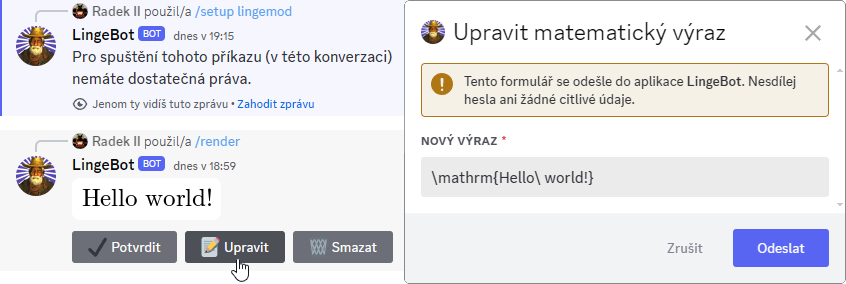
\includegraphics[width=.95\paperwidth]{img/idk}
	\end{frame}
	
	\begin{frame}\frametitle{Vykreslování matematických výrazů \texttt{/render}}
		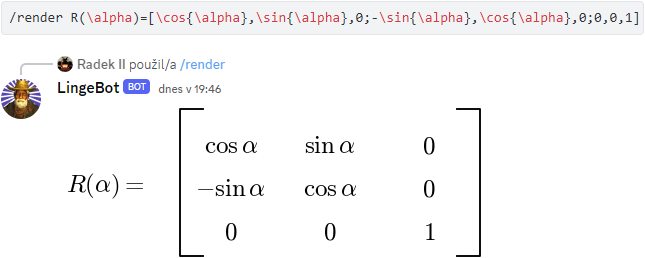
\includegraphics[width=.95\paperwidth]{img/idk2}
		\begin{itemize}
			\item Matplotlib Mathtext vs TeX
			\item Vykreslování matic a jejich zápis
			\item Rovnice s maticemi a aproximace délky výrazu
		\end{itemize}
	\end{frame}
	
	\begin{frame}\frametitle{Výklad teorie \texttt{/explain}}
		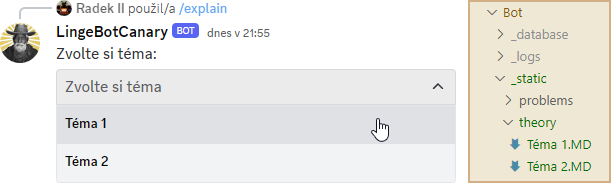
\includegraphics[width=.95\paperwidth]{img/idk3}
		\begin{itemize}
			\item Čtení z Markdown souborů
			\item „Hot reload“
			\item \texttt{\$\$\$render} $\to$ \texttt{/render}
			\item \texttt{<sub>} a \texttt{<sup>} $\to$ Unicode
			\item Obrázky přes internetový odkaz
		\end{itemize}
	\end{frame}
	
	\begin{frame}[plain]
		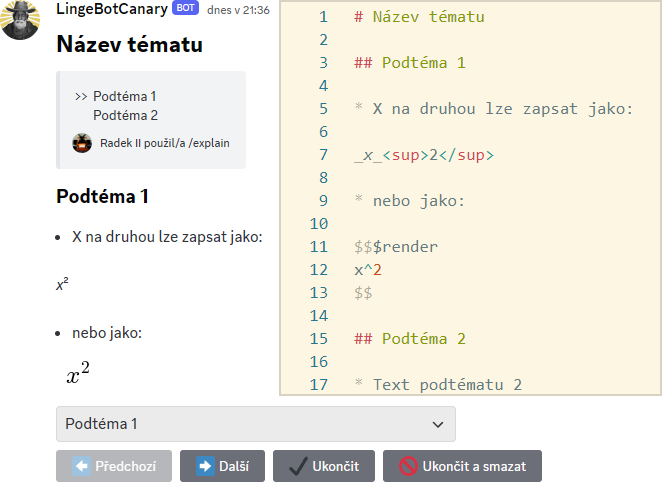
\includegraphics[width=.95\paperwidth]{img/idk4}
	\end{frame}
	
	\begin{frame}\frametitle{Generování příkladů \texttt{/generate}}
		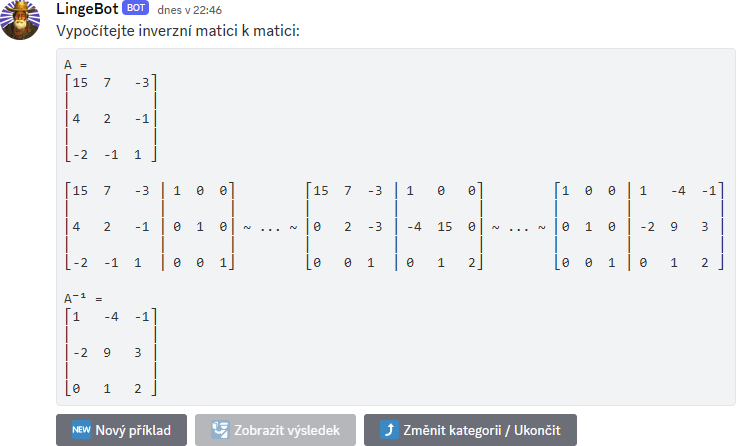
\includegraphics[width=.95\paperwidth]{img/idk5}
	\end{frame}
	
	\begin{frame}[plain]\frametitle{Diagram tříd generátoru příkladů}
		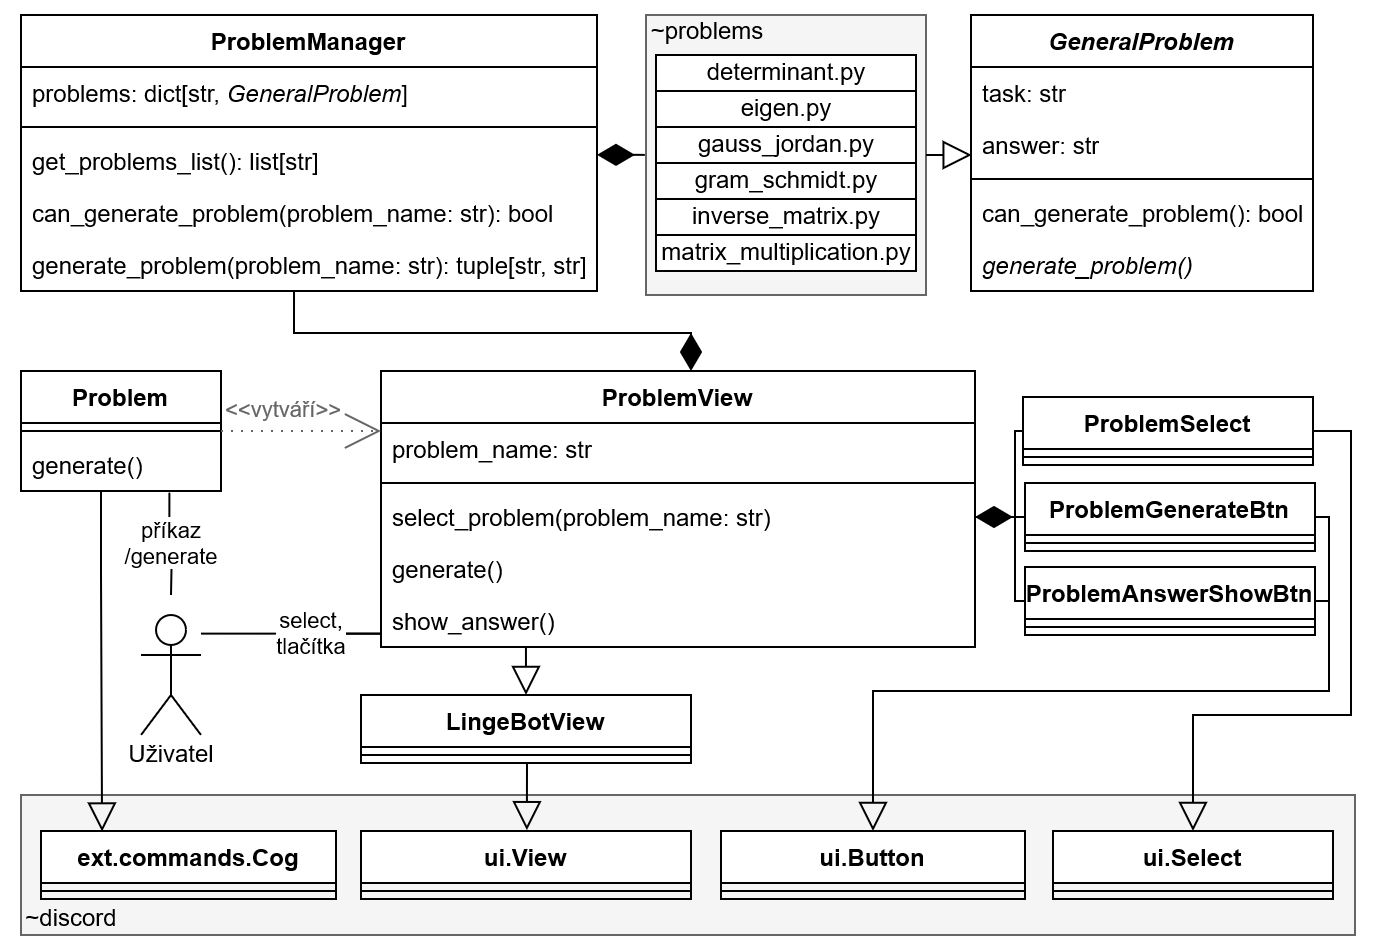
\includegraphics[width=.95\paperwidth]{img/idk6}
	\end{frame}
	
	\begin{frame}[plain]\frametitle{Sada příkazů \texttt{/setup}}
		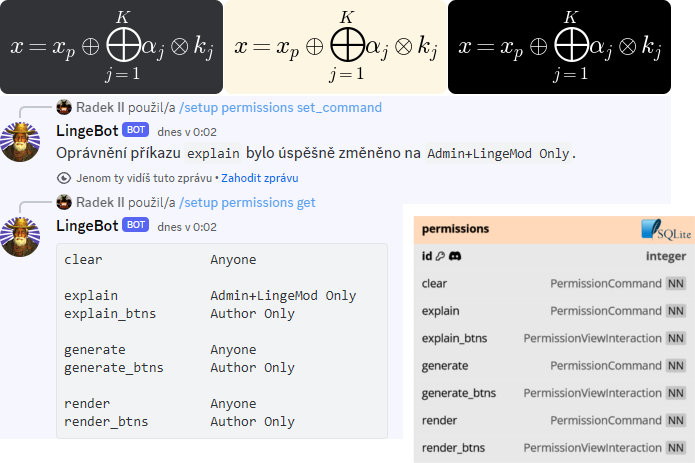
\includegraphics[width=.95\paperwidth]{img/idk7}
	\end{frame}
	
	\begin{frame}\frametitle{Závěr}
		\subheader{Shrnutí}
		\begin{itemize}
			\item Rešerše sociálních platforem podporujících boty
			\item Rešerše matematiky a knihoven pro tvorbu botů na Discordu
			\item Funkční bot
			\begin{itemize}
				\item \texttt{/render}, \texttt{/explain}, \texttt{/generate}
				\item Interaktivní prvky a oprávnění
				\item SQLite
				\item Možnost self-host, důraz na rozšiřitelnost
			\end{itemize}
			\item Ukázkové materiály
		\end{itemize}
		\subheader{Možná vylepšení}
		\begin{itemize}
			\item \texttt{/explain} – obrázky ze souboru a vyhledávání
			\item \texttt{/generate} – generovat sadu různých příkladů
			\item Lepší aproximace délky výrazu (\texttt{\textbackslash alpha} $\to$ 1, \texttt{\textbackslash sin} $\to$ 3, \dots)
			\item Použít SQLAlchemy
		\end{itemize}
	\end{frame}
	
	\TULendframe

	\begin{frame}[plain, noframenumbering]
		\bigskip
		„Zdůvodněte malý počet respondentů při získávání zpětné vazby.“
		\bigskip
		\begin{itemize}
			\item Uživatelská základna omezena na studenty ULA (TUL)
			\begin{itemize}
				\item Osloveno \textasciitilde100 lidí
				\item Větší důvěra v serióznost odpovědí
			\end{itemize}
			\item Nasazeno až během zkouškového období (pozdě)
		\end{itemize}
	\end{frame}
	
	\begin{frame}[plain, noframenumbering]
		\bigskip
		„Řešil jste nějakým způsobem mechanismus aktualizace bota vzhledem ke zmíněnému faktu, že platforma Discord je poměrně často aktualizována?“
		\bigskip
		\begin{itemize}
			\item Dvě instance bota – vývoj a produkce
			\item Nutno vylepšit Docker nasazení – bind mount
		\end{itemize}
	\end{frame}
	
	\begin{frame}[plain, noframenumbering]
		\bigskip
		„Mohl byste stručně shrnout, jak se Vámi navrhovaný bot liší od těch existujících, které v práci zmiňujete? V
		čem je Vaše řešení inovativní?“
		\bigskip
		\begin{itemize}		
		\item Zaměřením existujících botů jsou výpočty („kalkulačka“) a vykreslování matematických výrazů. Funkce výkladu teorie a generace složitějších příkladů jsou tedy na trhu Discord botů unikátní.
		\item Vykreslování není z pohledu uživatele nijak inovativní; maximálně modal pro editaci. Z pohledu kódu je „zajímavá“ implementace vykreslování matic bez použití KaTeX / MathJax.
		\end{itemize}
	\end{frame}
	
	\begin{frame}[plain, noframenumbering]
		\bigskip
		„Při hodnocení platformy Discord upozorňujete na problematiku aktualizací a potenciální změny v chování
		bota. Vzhledem k tomu, že k aktualizacím dochází jednou měsíčně, je Vámi navrhované řešení dlouhodobě
		udržitelné? Myslíte, že aktualizace můžou Vámi navrženého bota pravidelně měnit? Bude tedy potřeba každý
		měsíc do bota zasahovat?“
		\bigskip
		\begin{itemize}
			\item Poslední dobou jsou časté drobné kosmetické změny. Nejedná se ale o nic, co by narušilo funkce nebo čitelnost bota. V nejhorším případě musela být přepsána část Markdown materiálů – jediný zásah za půl roku.
			\item Problematičtější by mohly být aktualizace API, v zájmu Discordu by ale mělo být zachování zpětné kompatibility.
			\item Každá závislost je hrozbou (Discord, discord.py).
		\end{itemize}
	\end{frame}
	
\end{document}
